% One-pager: Same Storm, Different Boats
% Policy-oriented summary — AI-Econ Lab
% Compile with: tectonic onepager.tex

\documentclass[10pt,a4paper]{article}

% --- Packages ---
\usepackage[top=1.2cm, bottom=1.0cm, left=1.8cm, right=1.8cm]{geometry}
\usepackage{graphicx}
\usepackage[dvipsnames]{xcolor}
\usepackage{enumitem}
\usepackage{titlesec}
\usepackage{multicol}
\usepackage{paracol}
\usepackage{hyperref}
\usepackage[T1]{fontenc}
\usepackage{helvet}
\renewcommand{\familydefault}{\sfdefault}

% --- Colours ---
\definecolor{darkblue}{HTML}{1B3A5C}
\definecolor{orange}{HTML}{E8873A}
\definecolor{teal}{HTML}{2E7D6F}
\definecolor{lightgray}{HTML}{F0F0F0}
\definecolor{medgray}{HTML}{888888}

% --- Section formatting ---
\titleformat{\section}{\small\bfseries\color{darkblue}}{}{0pt}{}
\titlespacing{\section}{0pt}{4pt}{1pt}

% --- No page numbers ---
\pagestyle{empty}

% --- Hyperlinks ---
\hypersetup{colorlinks=true, urlcolor=teal, linkcolor=teal}

\begin{document}

% === LOGO BAR ===
\noindent
\begin{minipage}[c]{0.16\textwidth}
  
\includegraphics[height=0.95cm]{../assets/logos/orebro_logo.png}
\end{minipage}\hfill
\begin{minipage}[c]{0.13\textwidth}
  
\includegraphics[height=0.7cm]{../assets/logos/ratio_logo.png}
\end{minipage}\hfill
\begin{minipage}[c]{0.09\textwidth}
  
\includegraphics[height=0.7cm]{../assets/logos/ai_econ_lab_logo.png}
\end{minipage}\hfill
\begin{minipage}[c]{0.16\textwidth}
  
\includegraphics[height=0.45cm]{../assets/logos/wasphs_logo.png}
\end{minipage}\hfill
\begin{minipage}[c]{0.16\textwidth}
  
\includegraphics[height=0.7cm]{../assets/logos/aiscaf_logo.png}
\end{minipage}

\vspace{0.15cm}
\noindent\textcolor{darkblue}{\rule{\textwidth}{1.5pt}}

% === TITLE ===
\vspace{0.15cm}
\begin{center}
  {\large\bfseries\color{darkblue} Same Storm, Different Boats:\\[1pt]
  Generative AI and the Age Gradient in Hiring}
\end{center}

\vspace{0.02cm}
\begin{center}
  {\footnotesize \href{https://www.magnuslodefalk.com}{Magnus Lodefalk}\textsuperscript{a,b} \;\textbullet\;
  Lydia L\"othman\textsuperscript{a} \;\textbullet\;
  Michael Koch\textsuperscript{c} \;\textbullet\;
  Erik Engberg\textsuperscript{a,b}}\\[1pt]
  {\scriptsize\color{medgray}
  \textsuperscript{a}\"Orebro University \quad
  \textsuperscript{b}RATIO Institute \quad
  \textsuperscript{c}Aarhus University / Kiel Institut}
\end{center}

\vspace{0.04cm}
\noindent\textcolor{darkblue}{\rule{\textwidth}{0.4pt}}

% === KEY FINDING BOX ===
\vspace{0.08cm}
\noindent
\colorbox{lightgray}{%
  \parbox{\dimexpr\textwidth-2\fboxsep}{%
    \vspace{3pt}
    \centering\small
    {\bfseries\color{darkblue} Key finding:}
    After ChatGPT's launch, employment of \textbf{\textcolor{orange}{22--25 year olds}}
    in AI-exposed occupations began declining relative to less exposed
    occupations, reaching \textbf{\textcolor{orange}{$-$5.5\%}} by early 2025,
    while employment of \textbf{\textcolor{teal}{workers over~50}} \textbf{\textcolor{teal}{rose by~1.3\%}}.
    The gap is accelerating.
    \vspace{3pt}
  }%
}

% === FIGURE ===
\vspace{0.08cm}
\begin{center}
  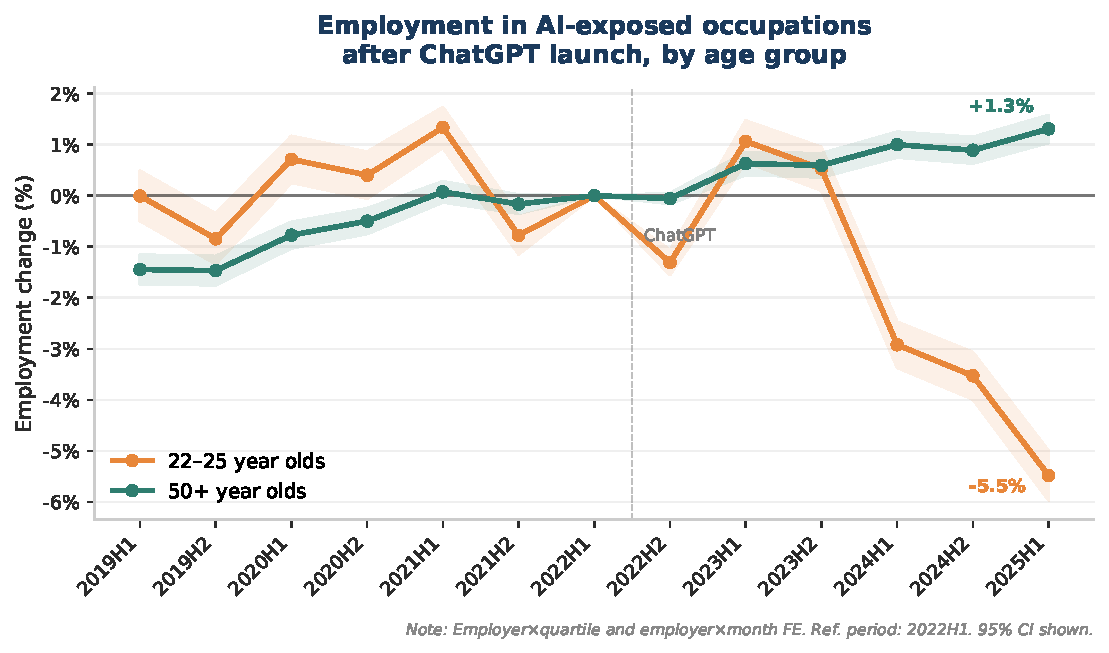
\includegraphics[width=0.74\textwidth]{../figures/onepager_age_gradient.pdf}
\end{center}

% === TWO COLUMNS: FINDINGS + POLICY ===
\vspace{-0.35cm}
\begin{multicols}{2}

\section{What we found}
\begin{itemize}[leftmargin=*, itemsep=1pt, parsep=0pt, topsep=0pt]
  \item The widely noted decline in job postings reflects
        \textbf{monetary tightening}, not AI. A natural timing test confirms
        this: the decline begins with the Riksbank rate hike (April 2022),
        seven months \emph{before} ChatGPT, and there is no correlation
        between AI exposure and interest-rate sensitivity.
  \item Beneath this aggregate null, however, AI \textbf{appears to be
        reshaping who gets hired}: within the same firms, young workers
        in AI-exposed occupations (e.g., software developers, customer
        service agents, administrative assistants) are disproportionately
        losing employment. \textbf{This compositional shift is invisible
        in posting data} and requires employer-level register data to detect.
  \item The effect \textbf{accelerates over time}: by early 2025,
        22--25 year olds in high-AI occupations had lost \textbf{5.5\%}
        of employment relative to low-AI occupations, up from near zero
        at launch. Workers aged 26--30 follow a similar trajectory
        ($-$4.9\% by 2025H1). Meanwhile, workers over~50 \emph{gained}
        1.3\%. The result mirrors US findings (Brynjolfsson et al., 2025)
        and contrasts with a Finnish null (Kauhanen, 2025); our
        within-employer design using \textbf{full-population} data
        may capture composition shifts not visible at the occupation level.
  \item The effect is \textbf{stronger for women}: the average
        post-ChatGPT effect for young women is $-$1.6\%, more than double
        the $-$0.7\% for young men.
  \item \textbf{Caveat:} Pre-trend tests reject formally, but for the
        core age groups the pre-trend direction is \emph{positive}
        (opposite to the finding), so trend extrapolation works
        against the result. A Rambachan-Roth sensitivity analysis
        is in progress.
\end{itemize}

\section{Policy implications}
\begin{itemize}[leftmargin=*, itemsep=1pt, parsep=0pt, topsep=0pt]
  \item \textbf{AI appears to operate on employment composition}, not only aggregate
        demand. If confirmed, targeted interventions are needed alongside broader
        economic policy.
  \item Candidate responses include \textbf{entry-level transition
        pathways}: vocational education (YH) and apprenticeships
        integrating AI tools, though their effectiveness for this
        specific challenge remains to be tested.
  \item \textbf{The silver lining}: evidence shows young workers recover
        faster from displacement than older workers (Athey et al., 2024),
        making early intervention particularly promising.
  \item Monitoring the \textbf{composition} of employment, not just
        the volume, is essential for timely policy response.
\end{itemize}

\end{multicols}

% === FOOTER ===
\vspace{-0.1cm}
\noindent\textcolor{darkblue}{\rule{\textwidth}{0.4pt}}
\vspace{0.04cm}

\noindent
{\scriptsize\color{medgray}
\textbf{Data \& method:} Monthly employer declarations (arbetsgivardeklarationer, AGI) from
Statistics Sweden, covering \emph{every} employment relationship in Sweden, 2019--June 2025.
Outcome: employment positions by age group and occupation.
AI exposure measured using the DAIOE index
(Engberg et al., 2024). Difference-in-differences with employer$\times$quartile
and employer$\times$month fixed effects, following Brynjolfsson et al.\ (2025).
SEs clustered by employer$\times$quartile.
DAIOE is constructed from pre-2022 work content, fixed across the sample period.
\hfill \textbf{16 March 2026}\\[1pt]
\hfill Code: \href{https://github.com/Magnus-L/canaries-sweden}{github.com/Magnus-L/canaries-sweden}}

\vspace{0.04cm}
\noindent
{\scriptsize\color{medgray}
\textit{\href{https://www.ai-econlab.com/papers}{Working paper}.
Part of \href{https://www.aiscaf.se/w/ac/}{AISCAF} (\href{https://wasp-hs.org}{WASP-HS}) and the \href{https://www.ai-econlab.com}{AI-Econ Lab} at \href{https://www.oru.se}{\"Orebro University} and \href{https://ratio.se}{Ratio}.}}

\noindent
{\scriptsize\color{medgray}
\textbf{Contact:}
Lydia L\"othman, \href{mailto:lydia.lothman@oru.se}{lydia.lothman@oru.se}, 070-9584726
\;\textbullet\;
Magnus Lodefalk, \href{mailto:magnus.lodefalk@oru.se}{magnus.lodefalk@oru.se}, 0722-217340}

\end{document}
